\chapter{Decision making}
The decision making component generates 8 poses evenly distributes on an sphere of radius 0.5 meters always with the viewpoint at the center of the sphere. As the object is not static in the scene, the center of the sphere can be moved by an interactive marker as shown on figure \ref{fig:robot_moving_around_object}. The poses are executed by the planner, and when the desired pose has been reached a message is be passed to the sensor nodes to do a capture.


\begin{figure}[htb]
	\begin{center}
		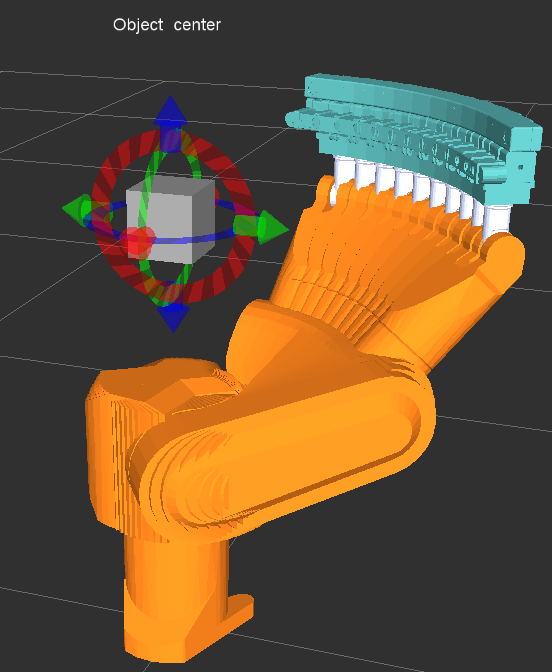
\includegraphics[scale=0.5,trim=0 0 0 0]{graphics/04_decisionmaking/robot_moving_around_object.png}%trim=l b r t
		\caption{The spin center is moveable by an interactive marker. The robot has planned a path to the next desired pose}
		\label{fig:robot_moving_around_object}
	\end{center}
\end{figure}

%\subsection{SMACH}
%SMACH = Next best view ready code
%state machine diagram?

\subsection{Special message type}
For easy offline manipulation of data a messagetype has been defined to carry the information acquired at each pose. Using this format allows the data to be captured at one point in time and processing at another by using rosbag between the nodes. Initially the message only contains the pose id, max number of poses and poses of the sensors, it is then passed on to the stereo camera node where the captured images are appended. Afterwards the dense\_stereo node creates and appends 3D information from the captured images and finally it can be passed to the reconstruction node.

\begin{figure}[htb]
	\begin{center}
		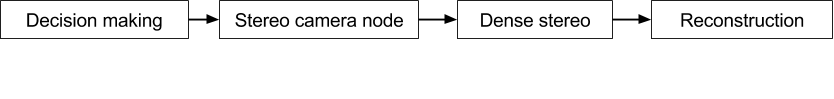
\includegraphics[scale=0.5,trim=0 50 0 0]{graphics/04_decisionmaking/message_path.png}%trim=l b r t
		\caption{The path of the message between the related nodes in the system. In each node new data is appended}
		\label{fig:message_path}
	\end{center}
\end{figure}

\subsection{State Machine}
The task is performed as a state machine (Figure \ref{fig:state_diagram}) consisting of two main states, move and capture. The move state executes a list of poses by issuing one pose at a time to the robot planner and wait for the robot state to reach within a threshold of the desired pose. Arriving at the pose transitions the state machine into the capture state, signalling the sensor node to collect data. Based on a time delay, the capture state transitions back to the move state. When the list of poses has all been executed, the move state remains at the final pose.


\begin{figure}[htb]
	\begin{center}
		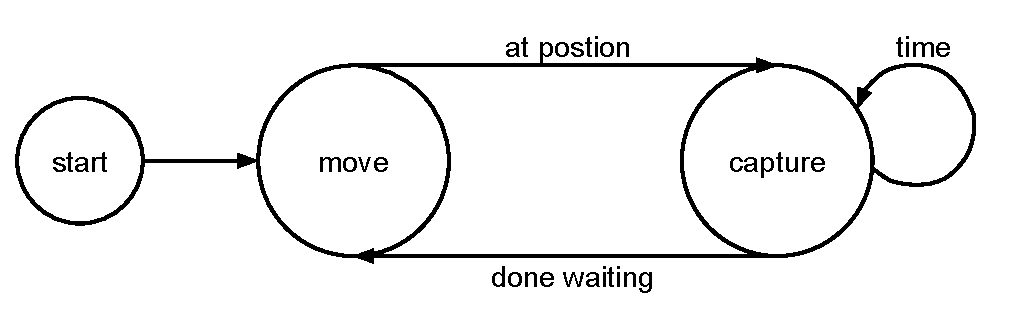
\includegraphics[scale=0.5,trim=0 0 0 0]{graphics/04_decisionmaking/state_diagram.pdf}%trim=l b r t
		\caption{State diagram of the decision maker}
		\label{fig:state_diagram}
	\end{center}
\end{figure}
